\subsection{Núcleo Via Láctea: Comunicação Institucional e Educacional}

\begin{figure}[!htbp]
\centering
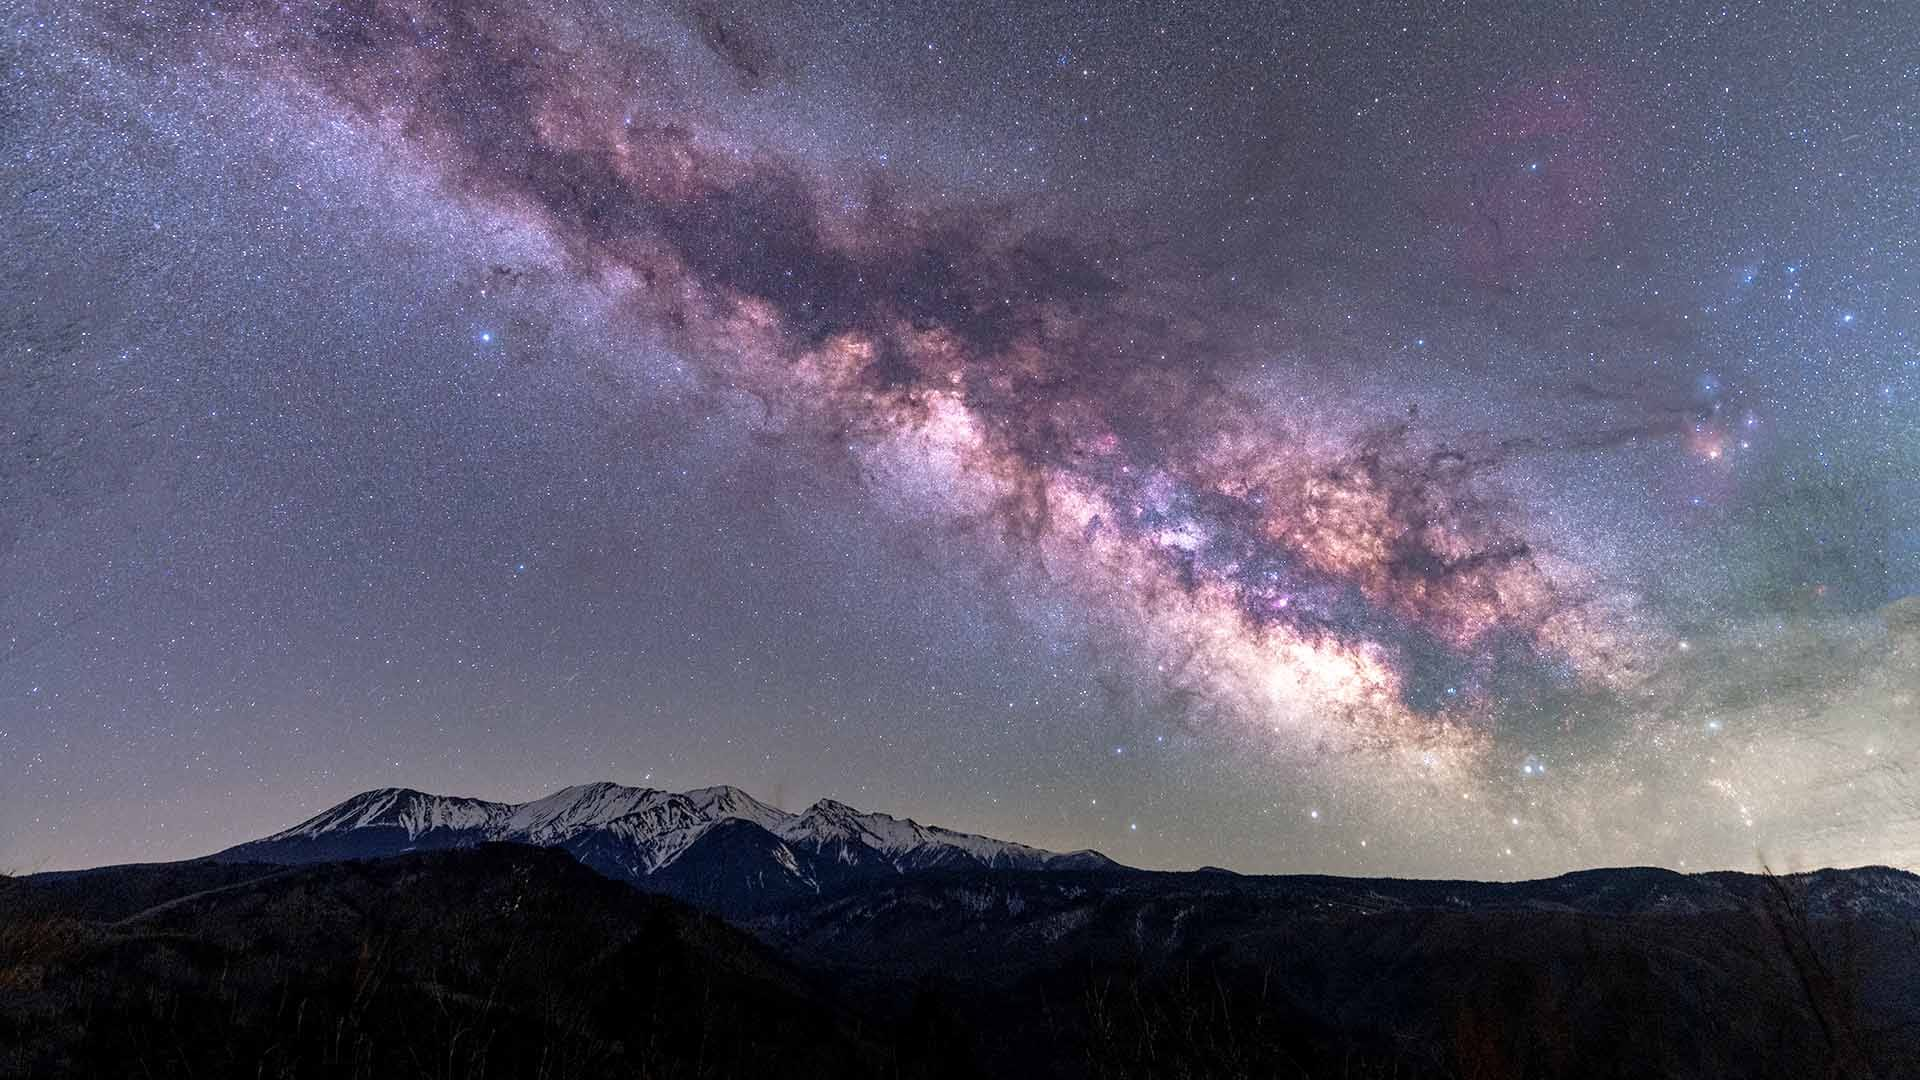
\includegraphics[width=1\linewidth]{files/vialactea-241d9e214ff4a2bcd2fd28d88f547093.jpg}
\end{figure}

\subsubsection{Visão Geral}

O \textbf{Núcleo Via Láctea} é responsável pelas ações de comunicação institucional e educacional do Projeto Hermathena. Seu nome evoca a nossa galáxia, simbolizando a base sólida sobre a qual se constrói toda a comunicação do projeto.

\subsubsection{Missão}

Estabelecer a identidade e a presença institucional do BINGO, produzir conteúdo educacional de qualidade e articular parcerias estratégicas com instituições formais.

\subsubsection{Objetivos Específicos}

\paragraph{1. Comunicação Institucional}

\subparagraph{1.1 Portal Web}

\begin{itemize}
\item[$\square$] Consolidar o portal \href{http://bingotelescope.org}{bingotelescope.org} como central de conteúdos
\item[$\square$] Implementar seção dedicada ao público brasileiro
\item[$\square$] Criar área de downloads para materiais educacionais
\item[$\square$] Estabelecer sistema de newsletter
\end{itemize}

\subparagraph{1.2 Identidade Visual}

\begin{itemize}
\item[$\square$] Desenvolver manual de identidade visual do Projeto Hermathena
\item[$\square$] Criar templates para documentos oficiais
\item[$\square$] Padronizar presença em eventos (banners, folders)
\item[$\square$] Implementar diretrizes de uso da marca BINGO
\end{itemize}

\subparagraph{1.3 Assessoria de Imprensa}

\begin{itemize}
\item[$\square$] Produzir press releases mensais
\item[$\square$] Manter banco de dados de jornalistas
\item[$\square$] Organizar coletivas de imprensa
\item[$\square$] Monitorar clipping de mídia
\end{itemize}

\paragraph{2. Comunicação Educacional}

\subparagraph{2.1 Material Didático}

\textbf{Para Ensino Fundamental (anos finais):}

\begin{itemize}
\item Cartilha ``O Universo em suas Mãos''
\item Jogos educativos sobre Sistema Solar
\item Posters astronômicos para sala de aula
\item Atividades práticas com materiais simples
\end{itemize}

\textbf{Para Ensino Médio:}

\begin{itemize}
\item Manual de Radioastronomia Básica
\item Roteiros de observação astronômica
\item Simulações computacionais
\item Propostas de experimentos
\end{itemize}

\textbf{Para Educadores:}

\begin{itemize}
\item Guia do Professor
\item Roteiros de aula estruturados
\item Sugestões de avaliação
\item Formação continuada
\end{itemize}

\subparagraph{2.2 Equipamentos de Demonstração}

\bigskip\noindent
\begin{tabular}{p{\dimexpr 0.333\linewidth-2\tabcolsep}p{\dimexpr 0.333\linewidth-2\tabcolsep}p{\dimexpr 0.333\linewidth-2\tabcolsep}}
\toprule
Equipamento & Descrição & Público-alvo \\
\hline
\textbf{Maquete do BINGO} & Modelo em escala 1:100 & Todos \\
\textbf{Radiolescópio didático} & Receptor de FM modificado & Ensino Médio \\
\textbf{Antena Hidrogeniana} & Receptor da linha de 21cm & Cursos técnicos \\
\textbf{Simulador de BAO} & Visualização de oscilações & Graduação \\
\textbf{Planetário portátil} & Projeção de constelações & Fundamental \\
\bottomrule
\end{tabular}

\bigskip

\subparagraph{2.3 Visitas e Experiências}

\begin{itemize}
\item \textbf{Visitas guiadas ao BINGO:} Protocolo de recebimento de escolas
\item \textbf{Roteiros de experiência:} Vivências práticas em radioastronomia
\item \textbf{Feiras de ciências:} Participação em eventos regionais
\item \textbf{Observações astronômicas:} Eventos noturnos com telescópios ópticos
\end{itemize}

\paragraph{3. Articulação Institucional}

\subparagraph{3.1 Parcerias Acadêmicas}

\bigskip\noindent
\begin{tabular}{p{\dimexpr 0.333\linewidth-2\tabcolsep}p{\dimexpr 0.333\linewidth-2\tabcolsep}p{\dimexpr 0.333\linewidth-2\tabcolsep}}
\toprule
Instituição & Tipo de Parceria & Ações Previstas \\
\hline
UEPB & Cooperação técnica & Divulgação no interior \\
IFPB & Cooperação técnica & Formação técnica \\
UFPB & Cooperação técnica & Pesquisa e extensão \\
USP & Colaboração BINGO & Suporte científico \\
INPE & Colaboração BINGO & Infraestrutura \\
\bottomrule
\end{tabular}

\bigskip

\subparagraph{3.2 Parcerias Governamentais}

\begin{itemize}
\item \textbf{SEECT-PB:} Integração com políticas estaduais de C\&T
\item \textbf{FAPESQ:} Cooperação em divulgação científica
\item \textbf{Prefeituras:} Ações em escolas municipais
\item \textbf{Secretarias de Educação:} Incorporação ao currículo
\end{itemize}

\subparagraph{3.3 Parcerias Privadas}

\begin{itemize}
\item Modelos: Patrocínio, mecenato, cooperação técnica
\item Setores prioritários: Telecom, energia, EdTech, turismo
\item Propostas personalizadas por segmento
\end{itemize}

\subsubsection{Metodologia}

\paragraph{Abordagem Educomunicativa}

Baseada nos princípios de:

\begin{enumerate}
\item \textbf{Diálogo horizontal:} Ciência como conversa, não imposição
\item \textbf{Contextualização:} Conectar conteúdo à realidade local
\item \textbf{Experimentação:} Aprender fazendo
\item \textbf{Colaboração:} Trabalho em rede
\end{enumerate}

\paragraph{Processo de Produção de Material}

\begin{verbatim}
┌─────────────┐    ┌─────────────┐    ┌─────────────┐    ┌─────────────┐
│  1. PESQUISA │ -> │ 2. ROTEIRO  │ -> │ 3. PRODUÇÃO │ -> │ 4. REVISÃO  │
│             │    │             │    │             │    │             │
│ Análise de  │    │ Estruturação│    │ Criação de  │    │ Validação   │
│ necessidades│    │ do conteúdo │    │ peças       │    │ com público │
└─────────────┘    └─────────────┘    └─────────────┘    └─────────────┘
                                                                │
                                                                v
┌─────────────┐    ┌─────────────┐    ┌─────────────┐    ┌─────────────┐
│ 8. ATUALIZA │ < - │ 7. AVALIAÇÃO│ < - │ 6. DIFUSÃO  │ < - │ 5. PUBLICAÇÃO│
│             │    │             │    │             │    │             │
│ Melhorias   │    │ Métricas de │    │ Distribuição│    │ Disponibili -│
│ contínuas   │    │ impacto     │    │ nos canais  │    │ zação formal│
└─────────────┘    └─────────────┘    └─────────────┘    └─────────────┘
\end{verbatim}

\subsubsection{Cronograma de Ações (Ano 1)}

\bigskip\noindent
\begin{tabular}{p{\dimexpr 0.250\linewidth-2\tabcolsep}p{\dimexpr 0.250\linewidth-2\tabcolsep}p{\dimexpr 0.250\linewidth-2\tabcolsep}p{\dimexpr 0.250\linewidth-2\tabcolsep}}
\toprule
Trimestre & Ação & Responsável & Produto \\
\hline
\textbf{T1} & Setup da infraestrutura & Coordenação & Estrutura operacional \\
\textbf{T1} & Desenvolvimento de identidade visual & Designer & Manual de marca \\
\textbf{T2} & Produção de material didático v1 & Equipe & 5 peças publicadas \\
\textbf{T2} & Primeiras visitas a escolas & Equipe & 3 escolas visitadas \\
\textbf{T3} & Workshop para educadores & Equipe & 20 participantes \\
\textbf{T3} & Feira de ciências regional & Equipe & Stand BINGO \\
\textbf{T4} & Avaliação e ajustes & Coordenação & Relatório de impacto \\
\bottomrule
\end{tabular}

\bigskip

\subsubsection{Indicadores}

\bigskip\noindent
\begin{tabular}{p{\dimexpr 0.333\linewidth-2\tabcolsep}p{\dimexpr 0.333\linewidth-2\tabcolsep}p{\dimexpr 0.333\linewidth-2\tabcolsep}}
\toprule
Indicador & Meta Ano 1 & Ferramenta de Medição \\
\hline
Materiais educacionais produzidos & 15 & Inventário \\
Escolas atendidas presencialmente & 10 & Registro de visitas \\
Educadores capacitados & 50 & Listas de presença \\
Downloads de materiais & 1.000 & Analytics \\
Parcerias institucionais firmadas & 5 & Acordos assinados \\
Releases publicados & 12 & Clipping \\
\bottomrule
\end{tabular}

\bigskip

\subsubsection{Estrutura da Equipe}

\bigskip\noindent
\begin{tabular}{p{\dimexpr 0.333\linewidth-2\tabcolsep}p{\dimexpr 0.333\linewidth-2\tabcolsep}p{\dimexpr 0.333\linewidth-2\tabcolsep}}
\toprule
Função & Quantidade & Perfil \\
\hline
\textbf{Professor Orientador} & 1 & Docente Física/Engenharia Elétrica \\
\textbf{Professor Colaborador} & 1 & Docente área complementar \\
\textbf{Bolsista PROBEX} & 1 & Graduação na área de afinidade \\
\textbf{Voluntários} & 5 & Graduação em áreas afins \\
\bottomrule
\end{tabular}

\bigskip

\textbf{Total por núcleo:} 8 pessoas

\textbf{Expansão:} Pode replicar em instituições parceiras (até 12 alunos + 4 docentes)

\subsubsection{Orçamento Estimado (Ano 1)}

\bigskip\noindent
\begin{tabular}{p{\dimexpr 0.500\linewidth-2\tabcolsep}p{\dimexpr 0.500\linewidth-2\tabcolsep}}
\toprule
Categoria & Valor (R\$) \\
\hline
Bolsa (1 bolsista $\times$ 6 meses $\times$ R\$ 400) & 2.400,00 \\
Material de consumo & 5.000,00 \\
Equipamentos de demonstração & 8.000,00 \\
Impressões gráficas & 3.000,00 \\
Deslocamentos & 5.000,00 \\
Eventos & 4.000,00 \\
\textbf{Total} & \textbf{33.400,00} \\
\bottomrule
\end{tabular}

\bigskip


\bigskip
\centerline{\rule{13cm}{0.4pt}}
\bigskip

\textit{Documento sujeito a revisões conforme evolução do projeto.}